\documentclass[11pt,a4paper]{article}
\usepackage[utf8]{inputenc}\usepackage[T1]{fontenc}
\usepackage[margin=1in]{geometry}
\usepackage{amsmath,amssymb,booktabs,graphicx,enumitem,xcolor,parskip,titlesec}
\usepackage[hidelinks]{hyperref}
\graphicspath{{figures/}}
\definecolor{qnavy}{RGB}{20,40,75}\definecolor{qgrey}{RGB}{90,90,90}\definecolor{qred}{RGB}{150,30,30}
\titleformat{\section}{\large\bfseries\color{qnavy}}{\thesection}{0.6em}{}
\begin{document}\thispagestyle{empty}
\noindent
{\large\bfseries\color{qnavy} Report R09 --- Can R06's Finding Be Replicated?}\\[2pt]
{\color{qgrey}Three attempts and a systematic screen of all 41 public lung cohorts. The answer
is no, and the reason is not the biology.}\\[6pt]
{\color{qgrey}\rule{\textwidth}{0.4pt}}

\medskip
\noindent 7 August 2026 \quad\textbullet\quad Quantara

\section*{Summary}

R06 reported that KEAP1 (HR 2.07) and SMARCA4 (HR 1.73) mutations are associated with shorter
overall survival in NSCLC, and its own audit \emph{withdrew} the accompanying replication claim:
the second cohort it tried had 45 events in 604 patients and failed its own positive controls.
That left the finding resting on a single cohort. This report is the attempt to fix that.

\textbf{It cannot be fixed with public data, and the blocker is measurable.} Three attempts:

\begin{enumerate}[leftmargin=1.4em,itemsep=2pt]
\item \textbf{TCGA-LUAD + LUSC} --- 978 patients, \textbf{385 events}, more than eight times the
      events of R06's failed attempt. Both positive controls still failed (TP53 HR 1.08,
      $q=0.67$; STK11 HR 1.52, $q=0.098$), in the full cohort \emph{and} in a pre-declared
      late-stage subgroup. Median OS is 50.3 months against 28.8 in R06's cohort: this is
      resected disease, not advanced disease.
\item \textbf{MSK metastatic-organotropism LUAD} --- rejected by a pre-registered setting gate
      before any hazard ratio was computed. Median OS 93.8 months, so despite the name it is not
      an advanced-disease cohort.
\item \textbf{A setting-matched pool} (NSCLC brain metastasis + a PDX-derived series, 380
      patients, \textbf{231 events}, median OS 29.7 and 24.7 months). Median survival now matches
      R06's setting closely --- and the controls fail again, with STK11 pointing the
      \emph{wrong way} (HR 0.85 against R06's 1.63).
\end{enumerate}

Between attempts, all 41 lung studies in cBioPortal were screened against five requirements
fixed in advance. \textbf{Two qualified.} Seventeen have no overall-survival endpoint at all,
fourteen have too few events, eight are the wrong disease setting.

\textbf{What this means, stated carefully.} This is not evidence that R06 is wrong. In every
cohort tested, mutations whose prognostic effect in NSCLC is well established --- TP53 and STK11
--- were also undetectable, so no cohort demonstrated the competence needed to test the
question. The honest conclusion is that \textbf{R06's finding remains a single-cohort result,
and no public dataset can currently adjudicate it.} \S5 specifies what would.

\section{Attempt 1 --- TCGA}

Model was R06's, unchanged: per-gene unadjusted Cox on overall survival, Benjamini--Hochberg
across the same five genes. Only patients in each study's \texttt{\_sequenced} list were used;
a patient without mutation profiling is not wild-type, and counting them as such would drag
every hazard ratio toward 1.

\begin{center}
\begin{tabular}{@{}lrrrr@{}}
\toprule
\textbf{Gene} & \textbf{Mutated} & \textbf{HR} & \textbf{$q$ (BH)} & \textbf{R06's HR} \\
\midrule
KEAP1   & 140 & 1.02 & 0.88 & 2.07 \\
SMARCA4 & \phantom{0}59 & 1.30 & 0.48 & 1.73 \\
KMT2D   & 145 & 1.09 & 0.67 & --- (n.s.) \\
\midrule
\textit{control} TP53  & 658 & 1.08 & 0.67 & 1.25 \\
\textit{control} STK11 & \phantom{0}77 & 1.52 & 0.098 & 1.63 \\
\bottomrule
\end{tabular}
\end{center}

\noindent 978 patients, 385 events, median OS 50.3 months.

STK11 is the near-miss worth noting: HR 1.52 against R06's 1.63 --- almost the same effect size
--- but $q=0.098$. TP53 is essentially absent. In the pre-declared late-stage (II--IV) subgroup
(468 patients, 222 events), TP53 actually inverts to HR 0.79, which is biologically implausible
and a clear signal that survival in this cohort is dominated by resection, adjuvant treatment
and competing risks rather than by primary-tumour mutation status.

Because both controls failed in both strata, the pre-registered rule halted the run. That halt
\emph{is} the result: TCGA cannot test this question, despite having ample events.

\section{The screen}

Rather than stop after two failures, all 41 lung studies in cBioPortal were screened on
requirements decided before any hazard ratio was computed: an OS endpoint; mutation profiling;
at least 100 events; median OS nearer R06's 28.8 months than TCGA's 50.3; and patients disjoint
from R06's cohort.

\begin{center}
\begin{tabular}{@{}lr@{}}
\toprule
No overall-survival endpoint & 17 \\
Fewer than 100 events & 14 \\
Wrong disease setting (median OS too long) & \phantom{0}8 \\
\textbf{Eligible} & \phantom{0}\textbf{2} \\
\midrule
Total screened & 41 \\
\bottomrule
\end{tabular}
\end{center}

The screen computes no outcome, only eligibility, so it cannot have been steered by results.

\begin{center}
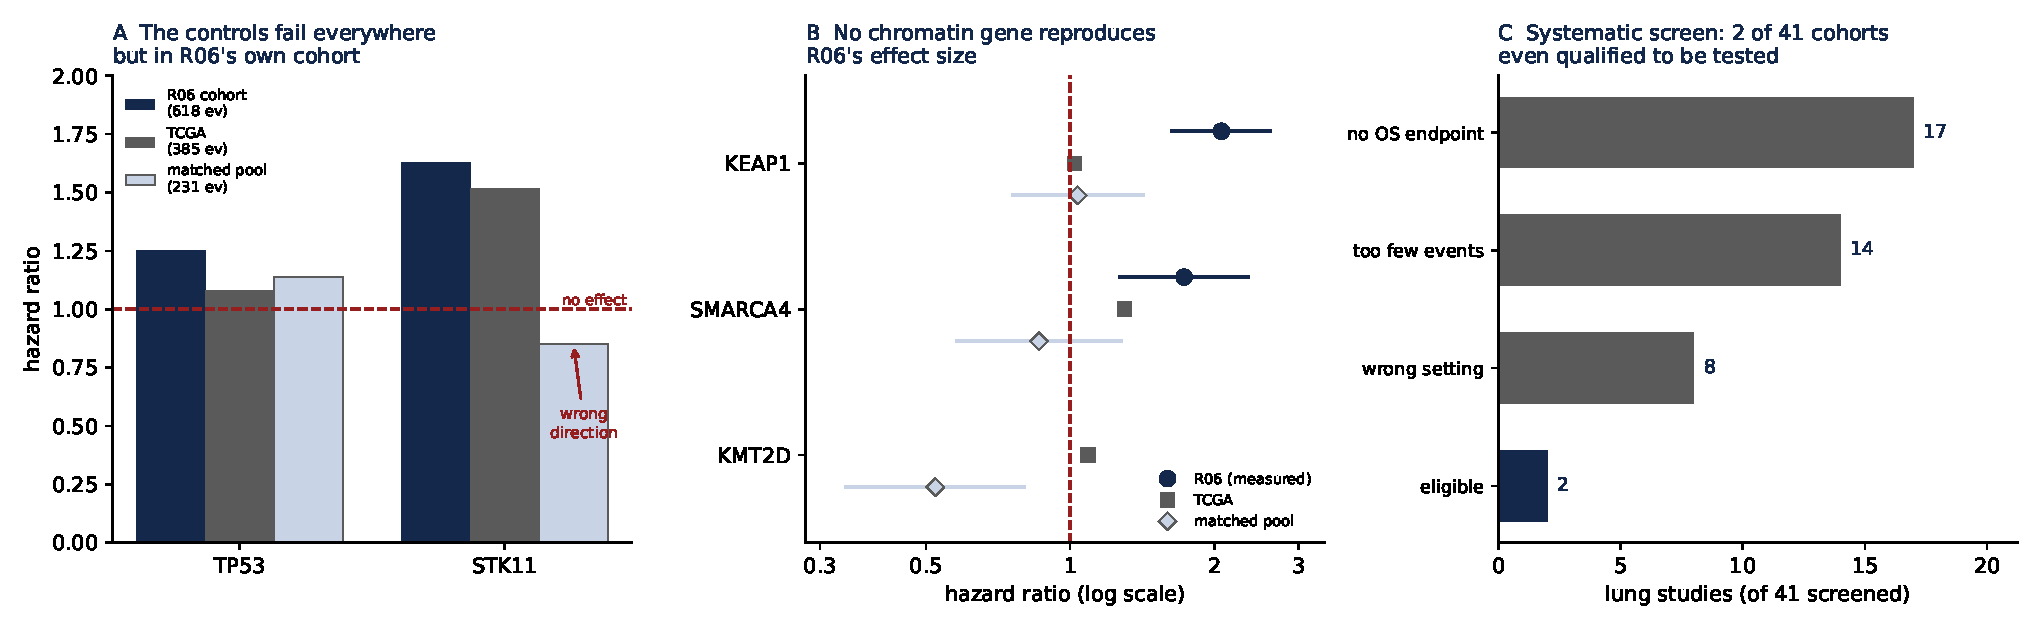
\includegraphics[width=\textwidth]{r09_panels.pdf}
\end{center}
\noindent{\small\color{qgrey}\textbf{A} The two positive controls in R06's cohort and in both
attempts. Neither reproduces outside R06's own data, and STK11 inverts in the matched pool.
\textbf{B} The three chromatin genes; R06's intervals are its measured 95\% CIs. \textbf{C} Why
there was nothing else to try.}

\section{Attempt 3 --- the setting-matched pool}

The two eligible cohorts: \texttt{bm\_nsclc\_mskcc\_2023} (NSCLC brain metastasis, 209 patients,
114 events, median OS 29.7 months) and \texttt{lung\_msk\_pdx} (171 patients, 117 events,
24.7 months). Twenty-four overlapping patients were removed from the first before any outcome
was read. Pooled analysis stratifies by cohort, so every comparison stays within-cohort and the
two very different selections are never contrasted with each other.

Power was computed \emph{before} running, so the control rule could not be rationalised
afterwards: at 231 events STK11's HR 1.63 corresponds to $z\approx2.6$ and should fire, while
TP53's HR 1.25 gives $z\approx1.7$ and may not. STK11 was therefore designated the load-bearing
control.

\begin{center}
\begin{tabular}{@{}lrrcr@{}}
\toprule
\textbf{Gene} & \textbf{Mutated} & \textbf{HR} & \textbf{95\% CI} & \textbf{$q$ (BH)} \\
\midrule
KEAP1   & \phantom{0}89 & 1.04 & 0.76--1.42 & 0.82 \\
SMARCA4 & \phantom{0}49 & 0.86 & 0.58--1.28 & 0.58 \\
KMT2D   & \phantom{0}52 & 0.52 & 0.34--0.80 & \textbf{0.014} \\
\midrule
\textit{control} TP53  & 269 & 1.14 & 0.85--1.51 & 0.58 \\
\textit{control} STK11 & \phantom{0}66 & 0.85 & 0.59--1.23 & 0.58 \\
\bottomrule
\end{tabular}
\end{center}

STK11 came out at 0.85 --- below 1, the opposite direction to R06's 1.63 --- so the load-bearing
control did not merely fail to reach significance, it pointed the wrong way. The run halted.

\textbf{The KMT2D row is why that halt matters.} It reaches $q=0.014$, and in a report without a
control gate it could have been written up as ``KMT2D mutation is protective in advanced NSCLC''.
It is not interpretable: it appears in cohorts that cannot reproduce established biology, it
contradicts R06 (which found KMT2D non-significant), it points in the protective direction, and
R08 separately showed KMT2D's apparent methylation phenotype was pure histology confounding.
Both of the strongest-looking KMT2D results in this series have dissolved on inspection.

\section{What would actually settle it}

Concretely, a cohort with all five of:

\begin{itemize}[leftmargin=1.2em,itemsep=2pt]
\item \textbf{Advanced or metastatic NSCLC}, median OS in the 20--35 month range. This is the
      binding constraint --- most public cohorts are surgically resected series.
\item \textbf{At least 250 deaths}, and preferably 400. Not merely 250 patients.
\item \textbf{Mutation calls} covering KEAP1, SMARCA4, KMT2D, STK11 and TP53.
\item \textbf{Patients disjoint} from \texttt{nsclc\_ctdx\_msk\_2022}.
\item \textbf{Ideally a different institution.} Both eligible cohorts here were MSK, as R06's
      was; disjoint patients are not institutional independence, and this report does not claim
      otherwise.
\end{itemize}

If the group holds or can access such a cohort, \texttt{evidence/m9\_tcga\_replication.py} runs
against it essentially unchanged --- the model, gates, controls and replication criterion are
fixed and hashed.

\textbf{A caution that cuts the other way.} Across three settings spanning 616 events, TP53 and
STK11 were undetectable, and STK11 inverted in one. That is a strong hint that
mutation--prognosis associations in NSCLC are highly dependent on disease setting and cohort
selection. R06's own result should be read with that in mind: it may be specific to
ctDNA-detected metastatic disease as sampled at one institution, rather than a general property
of NSCLC. R06 remains correctly reported as a single-cohort finding.

\section{Reproducing this report}

\begin{itemize}[leftmargin=1.2em,itemsep=1pt]
\item TCGA attempt: \texttt{evidence/m9\_tcga\_replication.py}; trace in
      \texttt{evidence/tcga\_*}, including \texttt{gates\_tcga\_FIRST\_HALT.json}
\item Screen: \texttt{evidence/screen\_replication\_cohorts.py} $\rightarrow$
      \texttt{evidence/screen\_results.json} (all 41 studies with per-study verdicts)
\item Matched attempt: \texttt{evidence/m10\_matched\_replication.py}; trace in
      \texttt{evidence/matched\_*}, plus
      \texttt{gates\_matched\_CANDIDATE\_REJECTED.json} for the cohort the setting gate rejected
\item Every number quoted above is consolidated in \texttt{evidence/consolidated.json}
\item Figure: \texttt{python3 make\_figure.py}
\item Data source: cBioPortal public REST API; no local data dependency
\end{itemize}

\end{document}
